42. \begin{figure}[ht!]
\center{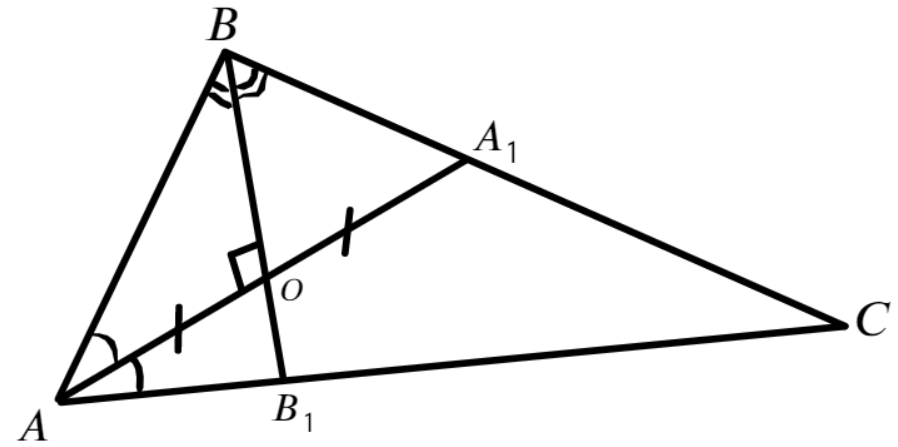
\includegraphics[scale=0.35]{g42.png}}
\end{figure}\\
Пусть биссектриса $BB_1$ поделила биссектрису $AA_1$ пополам. Тогда в треугольнике $ABA_1$ биссектриса $BO$ является медианой, а значит он равнобедренный и она является также и высотой. Но тогда $\angle BAO+\angle ABO=90^\circ\Rightarrow \angle A+\angle B=180^\circ,$ что невозможно.\\
